% HFUT_Courge_Project
\documentclass[UTF8]{ctexart}
\usepackage{fancyhdr}
\usepackage{graphicx}
\usepackage{titlesec}
\usepackage{titletoc}
\usepackage{listings}
\usepackage{appendix}
\usepackage{bm, amsmath,amsfonts}
\usepackage{multirow}
\usepackage[a4paper,left=3.4cm,right=3cm,top=1.65cm,bottom=2.54cm]{geometry}
\renewcommand{\contentsname}{\zihao{3} 目\quad 录}
\renewcommand{\abstractname}{\zihao{3} 摘\quad 要}
%页眉页脚设置
\pagestyle{fancy}
\fancyhf{}
\cfoot{\thepage}
\rhead{\kaishu~XX课程设计~}

%目录页设置
\titlecontents{section}[0em]{\zihao{4}\bf }{\thecontentslabel\ }{}
{\hspace{.5em}\titlerule*[4pt]{$\cdot$}\contentspage}
\titlecontents{subsection}[2em]{\vspace{0.1\baselineskip}\zihao{-4}}{\thecontentslabel\ }{}
{\hspace{.5em}\titlerule*[4pt]{$\cdot$}\contentspage}
\titlecontents{subsubsection}[4em]{\vspace{0.1\baselineskip}\zihao{-4}}{\thecontentslabel\ }{}
{\hspace{.5em}\titlerule*[4pt]{$\cdot$}\contentspage}
%代码设置
\RequirePackage{listings}
\RequirePackage{xcolor}
\definecolor{dkgreen}{rgb}{0,0.6,0}
\definecolor{gray}{rgb}{0.5,0.5,0.5}
\definecolor{mauve}{rgb}{0.58,0,0.82}
\lstset{
	numbers=left,  
	frame=tb,
	aboveskip=3mm,
	belowskip=3mm,
	showstringspaces=false,
	columns=flexible,
	framerule=1pt,
	rulecolor=\color{gray!35},
	backgroundcolor=\color{gray!5},
	basicstyle={\ttfamily},
	numberstyle=\tiny\color{gray},
	keywordstyle=\color{blue},
	commentstyle=\color{dkgreen},
	stringstyle=\color{mauve},
	breaklines=true,
	breakatwhitespace=true,
	tabsize=3,
}
%------------------------------------------------------------------------
%正文部分
\begin{document}
	\begin{titlepage}
		\centering
		\vspace*{1.75cm}
		\quad
\includegraphics[width=10.53cm,height=1.64cm]{hfut.jpg}\\
		\vspace*{1cm}
		{\fontsize{70pt}\baselineskip 课\qquad\ 程\qquad\ 设\qquad\ 计}
		 \vskip 7cm
		 \fontsize{19pt}\baselineskip
		 \makebox[30mm]{设计题目}
		 \underline{\makebox[75mm][c]{ 题目}}\\%在这里修改成自己的题目
		 \vskip 0.9cm
		 \makebox[30mm]{学生姓名}
		 \underline{\makebox[75mm][c]{ 姓名}}\\
		 \vskip 0.9cm
		 \makebox[30mm]{学\qquad\qquad 号}
		 \underline{\makebox[75mm][c]{ \LARGE 2016214000}}\\
		 \vskip 0.9cm
		 \makebox[30mm]{专业班级}
		 \underline{\makebox[75mm][c]{ 班级}}\\
		 \vskip 0.9cm
		  \makebox[30mm]{指导教师}
		 \underline{\makebox[75mm][c]{ 教师}}\\
		 \vskip 2cm
		 \LARGE \textbf{\number \year }~年~\textbf{\number\month}~月~\textbf{\number\day}~日		 
	\end{titlepage}

 \begin{abstract}
 	\pagestyle{plain}
 	\thispagestyle{empty}
 	\zihao{-4}
BP神经网络是一种具有反向修正功能的神经系统,具有的非线性特性和学习能力且已被证明具有逼近任意有界函数的能力。它有能力辨识那些不能线性化的非线性系统,不需要预先知道被测系统的模型。BP神经网络结构具有较强的自适应能力,并行处理和高度鲁棒性,采用神经网络方法设计的控制系统将具有更强的实时性,更强的适应能力和更强的鲁棒性。

随着无线通信技术的快速发展,互联网在人们的日常生活中占据了越来越重要的位置。网络中流量监控和预测对于研究网络拓扑结构有着重要的意义。本文参考BP算法,通过分析算法的优势和存在的一些问题,针对这些缺陷进行了改进。通过建立新的流量传输的传递函数,对比了经典的传递函数,并且在网络中进行了流量预测的实验和验证。新方法在试验中表现出了良好的实验性能,在网络流量预测中有很好的应用,可以作为网络流量预测的一个新方法和新思路,并且对研究网络拓扑结构有着重要的启发作用。网络流量预测在研究网络行为方面有着重要的作用。ARMA时间序列模型是比较常见的用于网络流量预测的模型。但是用在普通时间序列模型里面的一些参数很难估计,同时非固定的时间序列问题用ARMA模型很难解决。人工神经网络技术通过对历史数据的学习可能对大量数据的特征进行缓存记忆,对于解决大数据的复杂问题很合适。IP6网络流量预测是非线性的,可以使用合适的神经网络模型进行计算。	
	\\[0.5cm]
	\textbf{关键字}:\quad 关键字 \quad 关键字 \quad 关键字 \quad 关键字
	\newpage
\end{abstract}

\tableofcontents\thispagestyle{empty}
\newpage
\setcounter{page}{1}
\section{引言}
传统的系统辨识方法有着很多的不足,主要表现在:它要求研究人员给出系统模型的结构及阶次,即模型的建立要立足于函数的求解,这个过程是很难实现,因此确定模型参数的系统辨识理论的研究和应用都还局限于线性系统。人工神经网络是由大量而简单的神经元按某种方式连接形成的智能仿生动态网络,依靠计算机强大处理能力来实现对信息的处理。其具有的非线性特性和学习能力,为解决复杂的非线性、不确定系统的辨识问题,开辟了一条有效的途径。它不需要预先知道被测系统的模型就可以将系统模型辨识出来,这是神经网络辨识的优势所在。

人工神经网络是近年来的热点研究领域,涉及到电子科学与技术、信息与通信工程、计算机科学与技术、控制科学与技术等很多学科,其应用领域包括:建模、时间序列分析、模式识别和控制等,并在不断的拓展。神经网络的学习算法一直是人工神经网络理论研究和应用领域中一个重要的研究领域。神经网络的学习算法一直是人工神经网络理论研究和应用领域中的一个重要研究内容,尤其是对前馈神经网络学习算法的研究,至今没有一个十分理想的解决办法。其中BP神经网络在前馈神经网络学习算法中有着最广、最具有代表性。通过对BP神经网络算法较为深入的研究,提出了改进算法。

随着IPV6[14]的广泛应用,地址空间扩展到128位,网络结构变得越来越复杂。这就导致网络管理和运营出现了新的问题。网络流量通过建立网络流量模型,采用历史的数据可以预测网络中一段时间内的未来流量变化。一个好的模型不仅能够准确地反映历史数据的特性,并且能够预测未来一段时间内的网络流量。因此根据不同的网络特性,建立高效的网络流量模型对于网络流量的预测有着十分重要的意义。

和IPV4相比,IPV6网络有很多的新特性,比如说:多媒体流量和IPV6拓扑结构下的大量的有规律的数据流。因此,进行IPV6结构下的网络流量预测需要建立新的模型,使流量预测更加准确。人工神经网络技术广泛的应用到IPV4中进行流量预测,但是这些传统的网络模型通常都是假设网络中流量是线性的,使用数组和线性递归技术描述系统。但是IPV6中的网络流量没有表现出明显的规律性,因为网络流量包含了很多的非线性因素。最近的研究研究表明,传统的时间序列模型,线性预测模型不能够解决复杂的非线性流量预测,在一定程度上影响了网络流量预测的结果。
\subsection{第一小节}
这是测试文字这是测试文字这是测试文字这是测试文字这是测试文字这是测试文字这是测试文字这是测试文字这是测试文字这是测试文字
\par 这是测试文字这是这是测试文字这是测试文字这是测试文字这是测试文字这是测试文字这是测试文字这是测试文字这是测试文字
\par 文字这是这是测试文字这是测试文字这是测试文字这是测试文字这是测试文字这是测试文字这是测试文字这是测试文字这是测试文字这是测试文字这是测试文字
\subsubsection{第一小小节}
这是测试文字这是测试文字这是测试文字这是测试文字这是测试文字这是测试文字这是测试文字这是测试文字这是测试文字这是测试文字这是测试文字这是测试文字这是测试文字
\section{系统辨识}
所谓辨识建模是从实验数据出发,根据辨识的目的以及对过程已有的验前知识,预先给出一个模型类(线性的、非线性的、定常的、时变的、连续的、离散的… )进行拟合。无论是基于算法的辨识还是基于神经网络的辨识方法,都应当考虑模型、输入信号、以及误差准则的选择这三个基本问题:
\subsection{模型的选择}
模型是在某种意义下对于实际系统的一种近似描述,正确选择模型依赖于模型的用途和兼顾其精确性和复杂性问题。如果所建立的模型是用于系统分析的,则所需的模型必须把精确性放在首位,此时模型可能变得比较复杂。若建立的模型主要用于实时控制,可忽略次要因素,只考虑其主要因素,使模型简单些。在建立实际系统模型时,由于存在精确性和复杂性的矛盾,则要找到解决矛盾的折衷方法。反映在选择多层网络模型上,由于隐层及其节点数的确定目前还没有理论上的明确指导,折衷的方法即体现在通过多次仿真实验,找出能在给定准则下逼近原系统的最简单的多层网络模型。
\subsection{输入信号的选择}
为了能够辨识实际系统,输入信号必须满足一定条件。第一,在辨识时间内,输入信号必须是持续激励的,即输入信号必须充分激励系统的所有模态,使系统所有的模态都在模型中得以体现。从频谱观点看,输入信号的频谱必须足以覆盖系统的频谱。第二,输入信号的最优设计问题,即设计输入信号使给定问题的辨识精度最高。反映在BP网上,训练样本的选择应能使训练好的网络对所有模式类的输出响应都比较接近于实际输出。常用的输入信号有白噪声或伪随机信号。
\subsection{误差准则的选择}
误差准则是用来衡量模型接近实际系统的标准,它通常表示为一个误差的泛函,记作$ J(\theta)=\sum^l_{i=1}f[e(k)] $式中,$ f(\cdot) $是$ e(k) $的函数,用得最多的是平方函数,即$ f[e(k)]=e^2(k) $
\section{BP神经网络}
BP网络是一种利用误差反向传播训练算法的神经网络,简称BP(Back Propogation)网络,结构图如图1所示,是一种有隐含层的多层前馈网络,系统地解决了多层网络中隐含单元连接权的学习问题。 如果网络的输入节点数为M、输出节点数为L,则此神经网络可看成是从M维欧氏空间到L维欧氏空间的映射。这种映射是高度非线性的。
\begin{figure}[htbp]
	\centering
	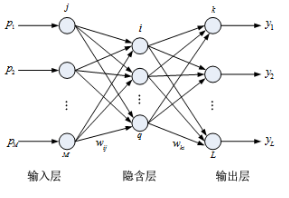
\includegraphics [width=0.3\textwidth]{fig/png1.png}
	\caption{BP神经网络结构图}
	\label{fig:my_png_1}
\end{figure}
\subsection{BP算法原理}
 BP学习算法的基本原理是梯度最速下降法,它的中心思想是调整权值使网络总误差最小。也就是采用梯度搜索技术,以期使网络的实际输出值与期望输出值的误差均方值为最小。网络学习过程是一种误差边向后传播边修正权系数的过程。这种学习的过程就是训练的过程,是神经网络各神经元连接方式、权值和阈值的调整过程,更是辨识的过程。学习的方法是使所确定的误差函数达到最小值,从而得到隐含在被测系统的输入输出数据之间的关系。

BP网络的每一层连接权值都可通过学习来调节。多层网络运行BP学习算法时,实际上包含了正向和反向传播两个阶段。在正向传播过程中,输入信息从输入层经隐含层逐层处理,并传向输出层,每一层神经元的状态只影响下一层神经元的状态。如果在输出层不能得到期望输出,则转入反向传播,将误差信号沿原来的连接通道返回,通过修改各层神经元的权值,使误差信号最小。

(1)信息的正向传递:
隐含层中第j个神经元的输出为
$$ y_{j}(n)=\varphi_j(\sum^{p}_{i=0}w_{ji}(n)y_i(n)) $$
对应于隐含层的函数$ \varphi_j(\cdot) $常常是S型激活函数
$$ y=\frac{1}{1-e^{-x}} $$
输出层第j个神经元的输出为
$$ y_j(n)=\psi_j(\sum^{p}_{i=0}w_{ji}(n)y_i(n)) $$
对应于输出层的函数$ \psi_j(\cdot) $常常是线性的激活函数。这是因为s型函数具有非线性放大系数功能,它可以把输入从负无穷大到正无穷大的信号,变换成-1到1之间输出,对较大的输入信号,放大系数较小;而对较小的输入信号,放大系数则较大,故可采用s型激活函数去处理和逼近非线性的输入、输出关系。不过,如果在输出层采用s型函数,输出则被限制到一个很小的范围了,若采用线性激活函数,则可使得网络输出任何值。所以只有希望对网络输出进行限制,才在输出层包含s型激活函数,而在一般情况下,均是在隐层采用s型激活函数,而在输出层采用线性激活函数。

第n个样本时,对应于第j个输出层神经元的误差信号是:
$$ e_j(n)=d_{j}(n)-y_j(n) $$
第n个样本时ide平方误差是:
$$ \xi(n)=\frac{1}{2}\sum^{p}_{j=0}e^{2}_{j}(n)  $$
平方误差的均值:
$$ \xi_{av}=\frac{1}{N}\sum^{N}_{n=1}\xi(n) $$
最终目的是让$ \xi_{av} $趋向最小。

(2)反向误差传播:
输出层的权值变化的公式如下:
$$ dw_{ji}(n)=-\eta\frac{\partial\xi(n)}{\partial w_{ji}(n)}=-\eta\cdot\delta_j(n)\cdot y_i(n) $$
其中:
$$ \delta_j(n)=(d_j(n)-y_j(n))\cdot \varphi_j(v_j(n)) $$
$$ v_j(n)=\sum^{p}_{i=0}w_{ji}(n)\cdot y_j(n) $$
隐含层的权值变化公式和输出层的类似,所不同的是,在这里:
$$ \delta_j(n)=\varphi_j(v_j(n))\cdot \sum_k(\delta_k(n)\cdot w_{kj}(n)) $$
其中,k表示的都是误差传播途径上的上一层神经元的量。

BP学习算法的基本原理是梯度最速下降法,它的中心思想是调整权值使网络总误差最小。 学习过程按使误差函数Jp减小最快的方向调整加权系数直到获得满意的加权系数为止。因此,权系数应按Jp函数梯度变化的反方向调整,使网络逐渐收敛。

输出层的神经元权系数修改公式:
$$ W_{k1}(k+1)=W_{k1}(k)+\eta\delta^{p}_{k}O^{p}_{k} $$
$$ \delta^{p}_{k}=o^{p}_{k}(1-o^{p}_{k})(t^{p}_{k}-o^{p}_{k})  $$
\subsection{改进的BP网络训练算法}
虽然BP网络有其重要地的意义,但在实际应用中存在不少问题:
\begin{itemize}
\item学习算法的收敛速度很慢。因为BP算法是以梯度下降法为基础的,只具有线性收敛速度,虽通过引入“势态项”增加了一定程度的二阶信息,但对算法的性质并无根本的改变。
\item学习因子和记忆因子    没有一种选择的规则,若选的过大会使训练的过程引起振荡,若选的过小会使训练的过程更加缓慢。
\item网络对初始值的敏感性。同一BP网络不同的初值会使网络的收敛速度差异很大。若初值权值离极小点很近,则收敛速度较快,若初值权值远离极小点,则收敛速度极慢。另外,若输入初值不合适,训练起始段就会出现振荡。
\item网络的隐层节点个数的选择尚无理论指导,而是根据经验选取。
\item从数学上看BP算法是一个非线性的优化问题,这就不可避免地存在局部极小问题。
\end{itemize}
\subsubsection{基于降低网络灵敏度的网络改进算法}






\subsubsection{第二小小节}
\par $a^2+b^2=c^2$
\[
a^2+b^2=c^2
\]
\begin{figure}[htbp]
	\centering
	\begin{minipage}[c]{0.5\textwidth}
		\centering
		
\includegraphics[width=0.3\textwidth]{test.jpg}
		\caption{测试1}
	\end{minipage}%
	\begin{minipage}[c]{0.5\textwidth}
		\centering
		
\includegraphics[width=0.3\textwidth]{test.jpg}
		\caption{测试2}
	\end{minipage}
\end{figure}
\section{表格}
\begin{table}[h]
	\caption{排序算法对比}
	\centering
	\begin{tabular}{||c|c|c|c|c|c||}
		\hline
		\multirow{2}*{类别}   &\multirow{2}*{排序方法} &\multicolumn{3}{|c|}{时间复杂度} &\multirow{2}*{稳定性}\\
		\cline{3-5}
		& &平均情况&最好情况&最坏情况& \\
		\hline
		\multirow{2}*{插入排序}&直接插入&$O(n^2)$&$O(n)$&$O(n^2)$&稳定\\
		\cline{2-6}
		&Shell排序&$O(n^{1.3})$&$O(n)$&$O(n^2)$&不稳定\\
		\hline
		\multirow{2}*{选择排序}&直接选择&$O(n^2)$&$O(n^2)$&$O(n^2)$&不稳定\\
		\cline{2-6}
		&堆排序&$O(n\log_{2}n)$&$O(n\log_{2}n)$&$O(n\log_{2}n)$&不稳定\\
		\hline
		\multirow{2}*{交换排序}&冒泡排序&$O(n^2)$&$O(n)$&$O(n^2)$&稳定\\
		\cline{2-6}
		&快速排序&$O(n\log_{2}n)$&$O(n\log_{2}n)$&$O(n^2)$& 不稳定\\
		\hline
		\multicolumn{2}{||c|}{归并排序}&$O(n\log_{2}n)$&$O(n\log_{2}n)$&$O(n\log_{2}n)$&稳定\\
		\hline
		\multicolumn{2}{||c|}{基数排序}&$d(r+n)$&$d(n+rd)$&$d(r+n)$& 稳定\\
		\hline
	\end{tabular}
\end{table}
\section{总结}
\par 这是测试文字这是测试文字这是测试文字这是测试文字这是测试文字这是测试文字这是测试文字这是测试文字这是测试文字这是测试文字这是测试文字这是测试文字这是测试文字这是测试文字这是测试文字这是测试文字这是测试文字这是测试文字这是测试文字这是测试文字这是测试文字这是测试文字这是测试文字这是测试文字这是测试文字这是测试文字这是测试文字这是测试文字这是测试文字这是测试文字这是测试文字这是测试文字这是测试文字这是测试文字这是测试文字这是测试文字这是测试文字这是测试文字这是测试文字这是测试文字这是测试文字这是测试文字这是测试文字这是测试文字这是测试文字这是测试文字这是测试文字这是测试文字这是测试文字这是测试文字这是测试文字这是测试文字这是测试文字这是
\par 测试文字这是测试文字这是测试文字这是测试文字这是测试文字这是测试文字这是测试文字这是测试文字这是测试文字这是测试文字这是测试文字这是测试文字这是测试文字这是测试文字这是测试文字这是测试文字这是测试文字这是测试文字这是测试文字这是测试文字这是测试文字这是测试文字这是测试文字这是测试文字这是测试文字这是测试文字这是测试文字这是测试文字这是测试文字这是测试文字这是测试文字这是测试文字这是测试文字这是测试文字这是测试文字这是测试文字这是测试文字这是测试文字这是测试文字这是测试文字这是测试文字这是测试文字这是测试文字这是测试文字这是测试文字这是测试文字这是测试文字这是测试文字这是测试文字这是测试文字这是测试文字这是测试文字这是测试文字这是测试文字这是测试文字这是测试文字这是测试文字这是测试文字这是测试文字这是测试文字这是测试文字这是测试文字这是测试文字这是测试文字这是测试文字这是测试文字这是测试文字这是测试文字这是测试文字这是测试文字这是测试文字这是测试文字这是测试文字这是测试文字这是测试文字这是测试文字这是测试文字这是测试文字这是测试文字这是测试文字这是测试文字这是测试文字这是测试文字这是测试文字这是测试文字这是测试文字这是测试文字
\par 这是测试文字这是测试文字这是测试文字这是测试文字这是测试文字这是测试文字这是测试文字这是测试文字这是测试文字这是测试文字这是测试文字这是测试文字这是测试文字这是测试文字这是测试文字这是测试文字这是测试文字这是测试文字这是测试文字这是测试文字这是测试文字这是测试文字这是测试文字这是测试文字这是测试文字这是测试文字这是测试文字
\newpage
\begin{appendices}
\section{程序代码}
\begin{lstlisting}[language=C++,escapeinside=``]
#include<iostream>
using namespace std;
int main
{
	cout<<"Hello world!"<<endl;//`输出`
	return 0;
}
\end{lstlisting}
\end{appendices}
	
\end{document}